
%(BEGIN_QUESTION)
% Copyright 2012, Tony R. Kuphaldt, released under the Creative Commons Attribution License (v 1.0)
% This means you may do almost anything with this work of mine, so long as you give me proper credit

Suppose you need to design a three-phase electric heater to dissipate 15 kW of heat when powered by 480 VAC.  Your options are to build a delta-connected heater array or a wye-connected heater array:

$$\includegraphics[width=15.5cm]{i01040x01.eps}$$

Calculate the proper resistance value for each array, to achieve the desired heat output:

\vskip 10pt

$R_{delta}$ = \underbar{\hskip 50pt} $\Omega$

\vskip 10pt

$R_{wye}$ = \underbar{\hskip 50pt} $\Omega$

\vskip 10pt

\underbar{file i01040}
%(END_QUESTION)





%(BEGIN_ANSWER)

Perhaps the simplest approach to this problem is to calculate the power dissipation of each resistor inside of each three-resistor array.  Since power is a scalar quantity (i.e. it adds directly, not trigonometrically), the 15 kW total heat output of each array means each resistor inside of each array must dissipate 5 kW of power.
 
\vskip 10pt

In the delta-connected heater, each resistor sees full line voltage (480 VAC), therefore the resistance may be calculated as such:

$$R = {V^2 \over P} = {480^2 \over 5000} = 46.08 \> \Omega$$

In the wye-connected heater, each resistor sees $1 \over \sqrt{3}$ of the full line voltage (480 VAC), which is 277.1 VAC.  Therefore the resistance may be calculated as such:

$$R = {V^2 \over P} = {277.1^2 \over 5000} = 15.36 \> \Omega$$

%(END_ANSWER)





%(BEGIN_NOTES)


%INDEX% Electronics review: 3-phase voltage/current/power calculation

%(END_NOTES)


